\documentclass[aspectratio=169,11pt]{beamer}

% Encoding
\usepackage[utf8]{inputenc}
\usepackage[T1]{fontenc}

% Theme
\usetheme{Madrid}
\usecolortheme{dolphin}
\setbeamertemplate{navigation symbols}{}
\setbeamertemplate{footline}[frame number]

% Graphics
\usepackage{graphicx}
\graphicspath{{./figures/}}

% TikZ
\usepackage{tikz}
\usetikzlibrary{arrows.meta, positioning, shapes.geometric, calc,
                 backgrounds, decorations.pathreplacing}

% Math
\usepackage{amsmath, amssymb}

% Tables
\usepackage{booktabs}

% Units
\usepackage{siunitx}
\usepackage{pifont}

% Colors
\definecolor{darkblue}{RGB}{0,75,135}
\definecolor{urjcblue}{RGB}{0,102,153}
\definecolor{alertred}{RGB}{204,0,0}
\definecolor{successgreen}{RGB}{0,128,0}
\definecolor{datablue}{RGB}{33,102,172}
\definecolor{nfgreen}{RGB}{27,120,55}
\definecolor{physred}{RGB}{178,24,43}
\definecolor{lightbg}{RGB}{240,245,255}
\setbeamercolor{structure}{fg=darkblue}

% Compact itemize
\setbeamertemplate{itemize items}[circle]
\setlength{\leftmargini}{1.2em}

% Custom commands
\newcommand{\kB}{k_{\mathrm{B}}}
\newcommand{\emphbox}[1]{\colorbox{blue!8}{\parbox{0.92\textwidth}{#1}}}
\newcommand{\smallemphbox}[1]{\colorbox{blue!8}{\parbox{0.42\textwidth}{#1}}}

% Metadata
\title[NF for Hidden Entropy]{Recovering Hidden Entropy Production\\via Normalizing Flows}
\subtitle{Continuous Density Estimation in Driven Langevin Dynamics}
\author{Antonio Fern\'{a}ndez-Caballero}
\institute{URJC -- LEADS / BigMed+}
\date{}

\begin{document}

% ============================================================================
% TITLE
% ============================================================================
\begin{frame}
\titlepage
\end{frame}

% ============================================================================
% HOOK
% ============================================================================
\begin{frame}{The Hidden Entropy Problem}

\begin{columns}[T]
\column{0.52\textwidth}
\textbf{Stochastic thermodynamics} quantifies irreversibility via the entropy production rate (EPR).

\smallskip
For a bistable system driven by a cyclic protocol:
\begin{itemize}
    \item \textbf{Sekimoto} (work--energy balance) $\to$ \textbf{100\%}
    \item \textbf{Schnakenberg} (L$\leftrightarrow$R transitions) $\to$ \textbf{$\sim$5\%}
\end{itemize}

\smallskip
\emphbox{\centering \textbf{$\sim$95\% of dissipation is ``hidden''} --\\invisible to coarse-grained descriptions.}

\column{0.45\textwidth}
\centering
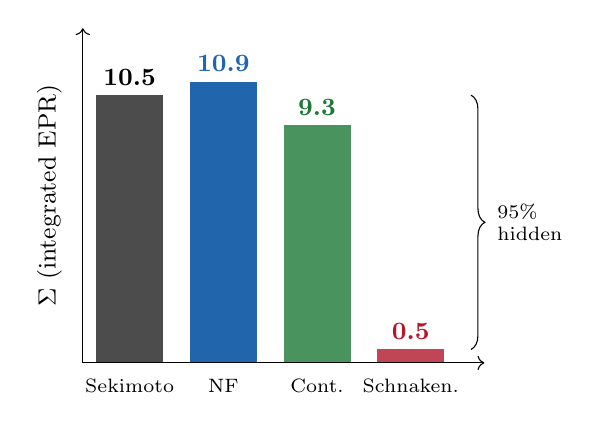
\begin{tikzpicture}[scale=0.85]
  % Bar chart comparing methods
  \fill[black!70] (0,0) rectangle (1.0,4.0);
  \fill[datablue] (1.4,0) rectangle (2.4,4.2);
  \fill[nfgreen!80] (2.8,0) rectangle (3.8,3.55);
  \fill[physred!80] (4.2,0) rectangle (5.2,0.2);
  % Labels
  \node[below,font=\scriptsize] at (0.5,-0.1) {Sekimoto};
  \node[below,font=\scriptsize] at (1.9,-0.1) {NF};
  \node[below,font=\scriptsize] at (3.3,-0.1) {Cont.};
  \node[below,font=\scriptsize] at (4.7,-0.1) {Schnaken.};
  % Values
  \node[above,font=\small\bfseries] at (0.5,4.0) {10.5};
  \node[above,font=\small\bfseries,color=datablue] at (1.9,4.2) {10.9};
  \node[above,font=\small\bfseries,color=nfgreen] at (3.3,3.55) {9.3};
  \node[above,font=\small\bfseries,color=physred] at (4.7,0.2) {0.5};
  % Axis
  \draw[->] (-0.2,0) -- (5.8,0);
  \draw[->] (-0.2,0) -- (-0.2,5.0);
  \node[rotate=90,font=\small] at (-0.7,2.5) {$\Sigma$ (integrated EPR)};
  % Brace for hidden
  \draw[decorate,decoration={brace,mirror,amplitude=5pt}] (5.6,0.2) -- (5.6,4.0)
    node[midway,right=6pt,font=\scriptsize,align=left] {95\%\\hidden};
\end{tikzpicture}
\end{columns}

\end{frame}

% ============================================================================
\begin{frame}{What is Entropy Production?}

\begin{columns}[T]
\column{0.50\textwidth}
\textbf{Physical intuition:}\\[0.3em]
Entropy production measures \textbf{irreversibility}---the thermodynamic ``cost'' of driving a system away from equilibrium.

\smallskip
\textbf{Everyday analogy:}\\
Stirring coffee dissipates work as heat.\\
The spoon's motion never spontaneously reverses.

\smallskip
\textbf{At the molecular scale:}\\
Irreversibility appears as \emph{probability currents} that violate detailed balance ($J \neq 0$).

\column{0.45\textwidth}
\centering
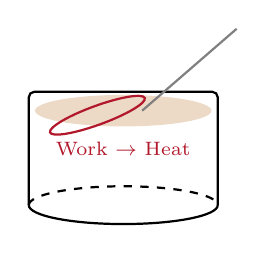
\begin{tikzpicture}[scale=0.8]
  % Coffee cup
  \draw[thick,rounded corners=2pt] (-1.5,-0.3) -- (-1.5,1.5) -- (1.5,1.5) -- (1.5,-0.3);
  \draw[thick] (-1.5,-0.3) arc (180:360:1.5 and 0.3);
  \draw[thick,dashed] (-1.5,-0.3) arc (180:0:1.5 and 0.3);
  % Coffee surface
  \fill[brown!30] (0,1.2) ellipse (1.4 and 0.25);
  % Stirring arrow
  \draw[-{Stealth},thick,physred,rotate=20] (0,1.2) ellipse (0.8 and 0.15);
  \node[font=\scriptsize,physred] at (0,0.6) {Work $\to$ Heat};
  % Spoon
  \draw[thick,gray] (0.3,1.2) -- (1.8,2.5);
\end{tikzpicture}

\vspace{0.3em}
{\small Work done by stirring\\dissipates irreversibly.}
\end{columns}

\vspace{0.5em}
\emphbox{
\centering
\textbf{EPR} = rate of entropy production = $\displaystyle\int \frac{J(x)^2}{D\,p(x)}\,dx$
}

\end{frame}

% ============================================================================
\begin{frame}{Outline}
\tableofcontents
\end{frame}

% ============================================================================
\section{Background}
% ============================================================================

\begin{frame}{The Driven Landau Potential}

\begin{columns}[T]
\column{0.52\textwidth}

\textbf{Bistable potential} with external tilt:
\begin{equation*}
    V(x,h) = x^4 - 2x^2 + h\,x
\end{equation*}

\begin{itemize}
    \item Two metastable wells at $x \approx \pm 1$
    \item Field $h(t) = h_{\max}\sin(2\pi t/\mathcal{T})$
    \item $\kB T = 0.5$, $\gamma = 1$, $N = \num{5000}$
\end{itemize}

\smallskip
\textbf{Langevin equation:}
\begin{equation*}
    \gamma\,dx = -V'(x,h)\,dt + \sqrt{2\gamma \kB T}\,dW
\end{equation*}

\column{0.45\textwidth}
\centering
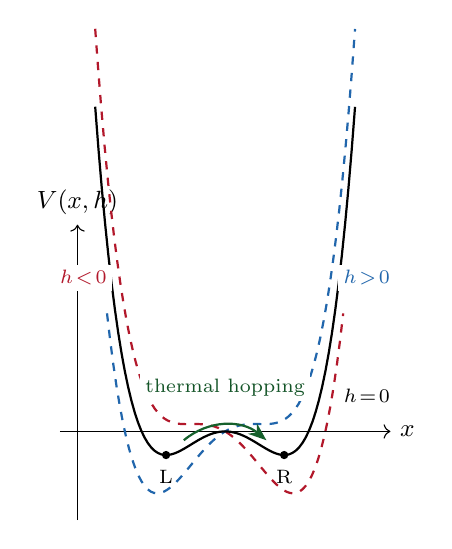
\begin{tikzpicture}[scale=0.75]
  % Axes
  \draw[->] (-2.8,0) -- (2.8,0) node[right,font=\small] {$x$};
  \draw[->] (-2.5,-1.5) -- (-2.5,3.5) node[above,font=\small] {$V(x,h)$};
  % V(x,0) — symmetric (draw last to be on top)
  % V(x,+1.5) — tilted right
  \draw[thick,datablue,dashed,domain=-2.0:2.2,samples=80]
    plot (\x, {0.4*(\x*\x*\x*\x - 2*\x*\x + 1.5*\x)});
  % V(x,-1.5) — tilted left
  \draw[thick,physred,dashed,domain=-2.2:2.0,samples=80]
    plot (\x, {0.4*(\x*\x*\x*\x - 2*\x*\x - 1.5*\x)});
  % V(x,0) — symmetric (on top)
  \draw[thick,black,domain=-2.2:2.2,samples=80]
    plot (\x, {0.4*(\x*\x*\x*\x - 2*\x*\x)});
  % Labels with white background, positioned clearly away from curves
  \node[font=\scriptsize,fill=white,inner sep=2pt] at (2.4,0.6) {$h\!=\!0$};
  \node[font=\scriptsize,fill=white,inner sep=2pt,text=datablue] at (2.4,2.6) {$h\!>\!0$};
  \node[font=\scriptsize,fill=white,inner sep=2pt,text=physred] at (-2.4,2.6) {$h\!<\!0$};
  % Well markers
  \fill[black] (-1.0,-0.4) circle (2pt);
  \fill[black] (1.0,-0.4) circle (2pt);
  \node[below,font=\scriptsize] at (-1.0,-0.5) {L};
  \node[below,font=\scriptsize] at (1.0,-0.5) {R};
  % Particle arrows
  \draw[-{Stealth},thick,nfgreen!80!black]
    (-0.7,-0.15) to[out=40,in=140] (0.7,-0.15);
  \node[above,font=\scriptsize,fill=white,inner sep=2pt,text=nfgreen!70!black] at (0,0.5) {thermal hopping};
\end{tikzpicture}

\vspace{0.3em}
{\small Sinusoidal $h(t)$ tilts the landscape,\\driving transitions between wells.}
\end{columns}

\end{frame}

% ============================================================================

\begin{frame}{Entropy Production Rate -- The Physics}

The \textbf{Fokker--Planck probability current} quantifies non-equilibrium flux:
\begin{equation*}
    J(x,t) = -\frac{V'(x,h)}{\gamma}\,p(x,t) - D\,\frac{\partial p}{\partial x}
\end{equation*}

The \textbf{local EPR density} measures irreversibility at each point:
\begin{equation*}
    \sigma(x,t) = \frac{J(x,t)^2}{D\,p(x,t)}
\end{equation*}

\smallskip
\emphbox{
\textbf{Key insight:} Computing $\sigma(x,t)$ requires the \textit{full density} $p(x,t)$ and its spatial derivative -- not just basin populations.
}

\smallskip
At equilibrium: $J \equiv 0 \implies \sigma \equiv 0$ (detailed balance).

\end{frame}

% ============================================================================

\begin{frame}{Three Ways to Estimate EPR}

\begin{columns}[c]
\column{0.30\textwidth}
\centering
\textbf{1. Sekimoto}\\[0.3em]
{\small (total, ground truth)}

\smallskip
$\displaystyle\dot{\Sigma}_{\mathrm{Sek}} = \frac{\langle x\rangle\,\dot{h} - \dot{E}}{\kB T}$

\smallskip
{\small Work--energy balance}\\
{\small Captures \textbf{all} dissipation}

\column{0.30\textwidth}
\centering
\textbf{2. Schnakenberg}\\[0.3em]
{\small (coarse-grained)}

\smallskip
$\displaystyle\dot{\Sigma}_{\mathrm{CG}} = \frac{J_{\mathrm{net}}}{\Delta t}\,\ln\frac{J_{01}}{J_{10}}$

\smallskip
{\small L$\leftrightarrow$R transitions only}\\
{\small Captures \textbf{$\sim$5\%}}

\column{0.30\textwidth}
\centering
\textbf{3. NF-EPR}\\[0.3em]
{\small (this work)}

\smallskip
$\displaystyle\dot{\Sigma}_{\mathrm{NF}} = \int \frac{J^2}{D\,p}\,dx$

\smallskip
{\small Learn $p(x,t)$ from data}\\
{\small Captures \textbf{$\sim$100\%}}
\end{columns}

\vspace{0.8em}
\emphbox{
\centering \textbf{Hidden entropy:}
$\Sigma_{\mathrm{hidden}} = \Sigma_{\mathrm{Sek}} - \Sigma_{\mathrm{CG}} \approx$ \textbf{95\%} of total dissipation
}

\end{frame}

% ============================================================================
\section{Normalizing Flows}
% ============================================================================

\begin{frame}{Normalizing Flows -- The Idea}

\centering
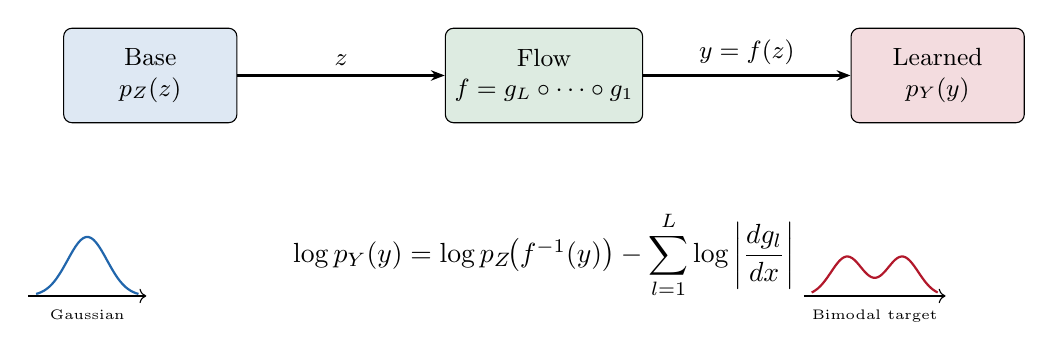
\begin{tikzpicture}[
    box/.style={draw,rounded corners=3pt,minimum width=2.2cm,minimum height=1.2cm,
                align=center,font=\small},
    arr/.style={-{Stealth[length=5pt]},thick}
]
  % Base distribution
  \node[box,fill=datablue!15] (base) at (0,0) {Base\\$p_Z(z)$};
  % Flow
  \node[box,fill=nfgreen!15] (flow) at (5,0) {Flow\\$f = g_L \circ \cdots \circ g_1$};
  % Target
  \node[box,fill=physred!15] (target) at (10,0) {Learned\\$p_Y(y)$};
  % Arrows
  \draw[arr] (base) -- (flow) node[midway,above,font=\small] {$z$};
  \draw[arr] (flow) -- (target) node[midway,above,font=\small] {$y = f(z)$};

  % Equation below
  \node[below=1.0cm of flow,font=\normalsize] (eq) {
    $\log p_Y(y) = \log p_Z\!\big(f^{-1}(y)\big) - \displaystyle\sum_{l=1}^{L} \log\left|\frac{dg_l}{dx}\right|$
  };

  % Small density sketches
  \begin{scope}[shift={(-0.8,-2.8)},scale=0.5]
    \draw[->] (-1.5,0) -- (1.5,0);
    \draw[thick,datablue,domain=-1.3:1.3,samples=40]
      plot (\x, {1.5*exp(-2*\x*\x)});
    \node[below,font=\tiny] at (0,-0.1) {Gaussian};
  \end{scope}
  \begin{scope}[shift={(9.2,-2.8)},scale=0.5]
    \draw[->] (-1.8,0) -- (1.8,0);
    \draw[thick,physred,domain=-1.6:1.6,samples=60]
      plot (\x, {1.0*exp(-3*(\x-0.7)*(\x-0.7)) + 1.0*exp(-3*(\x+0.7)*(\x+0.7))});
    \node[below,font=\tiny] at (0,-0.1) {Bimodal target};
  \end{scope}
\end{tikzpicture}

\vspace{0.3em}
\begin{itemize}
    \item Exact, differentiable density -- not a histogram or KDE
    \item Score $s(x) = \partial\log p/\partial x$ reconstructs the Fokker--Planck current
\end{itemize}

\end{frame}

% ============================================================================

\begin{frame}{NF Architecture Landscape (Kobyzev et al., 2021)}

\centering
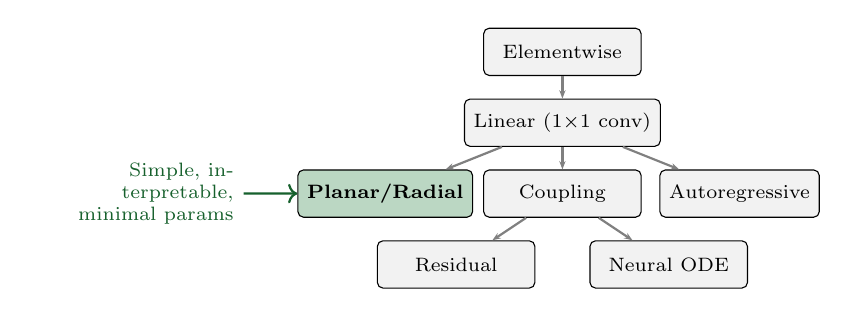
\begin{tikzpicture}[
    box/.style={draw,rounded corners=2pt,minimum width=2.0cm,minimum height=0.6cm,
                align=center,font=\scriptsize},
    arr/.style={-{Stealth[length=3pt]},thick,gray},
    scale=0.9
]
  % Hierarchy
  \node[box,fill=gray!10] (elem) at (0,3) {Elementwise};
  \node[box,fill=gray!10] (linear) at (0,2) {Linear (1$\times$1 conv)};
  \node[box,fill=nfgreen!30] (planar) at (-2.5,1) {\textbf{Planar/Radial}};
  \node[box,fill=gray!10] (coupling) at (0,1) {Coupling};
  \node[box,fill=gray!10] (ar) at (2.5,1) {Autoregressive};
  \node[box,fill=gray!10] (residual) at (-1.5,0) {Residual};
  \node[box,fill=gray!10] (ode) at (1.5,0) {Neural ODE};

  % Arrows
  \draw[arr] (elem) -- (linear);
  \draw[arr] (linear) -- (planar);
  \draw[arr] (linear) -- (coupling);
  \draw[arr] (linear) -- (ar);
  \draw[arr] (coupling) -- (residual);
  \draw[arr] (coupling) -- (ode);

  % Annotation
  \draw[thick,nfgreen!80!black,->] (-4.5,1) -- (planar.west);
  \node[left,font=\scriptsize,nfgreen!80!black,text width=2.5cm,align=right] at (-4.5,1)
    {Simple, interpretable,\\minimal params};
\end{tikzpicture}

\vspace{0.5em}
\begin{columns}[T]
\column{0.48\textwidth}
\textbf{Why planar flows?}
\begin{itemize}
    \item Only 3 params/layer
    \item Invertible via Newton
    \item Sufficient for 1D
\end{itemize}

\column{0.48\textwidth}
\textbf{Key limitation:}
\begin{itemize}
    \item Monotone composition
    \item Cannot create modes
    \item[$\to$] Need GMM base for bimodal
\end{itemize}
\end{columns}

\end{frame}

% ============================================================================

\begin{frame}{Planar Flow Architecture (1D)}

Each layer is a simple diffeomorphism:
\begin{equation*}
    g(x) = x + u\,\tanh(w\,x + b), \qquad
    \frac{dg}{dx} = 1 + u\,w\,\mathrm{sech}^2(w\,x + b)
\end{equation*}

\begin{columns}[T]
\column{0.52\textwidth}
\textbf{Properties:}
\begin{itemize}
    \item Monotone if $u\,w > -1$ (enforced)
    \item Compose $L$ layers: $f = g_L \circ \cdots \circ g_1$
    \item Only 3 parameters per layer
    \item Invert via Newton's method ($\mathrm{tol}=10^{-12}$)
\end{itemize}

\column{0.42\textwidth}
\centering
\textbf{Our configuration:}\\[0.3em]
\begin{tabular}{ll}
\toprule
Layers $L$ & 14 \\
Base & GMM ($K=2$) \\
Params/snapshot & 47 \\
Optimizer & L-BFGS-B \\
Time bins & 40 \\
\bottomrule
\end{tabular}

\smallskip
{\small Pure NumPy/SciPy\\(no PyTorch, no AD)}
\end{columns}

\end{frame}

% ============================================================================

\begin{frame}{Why Standard Normal Base Fails}

\centering
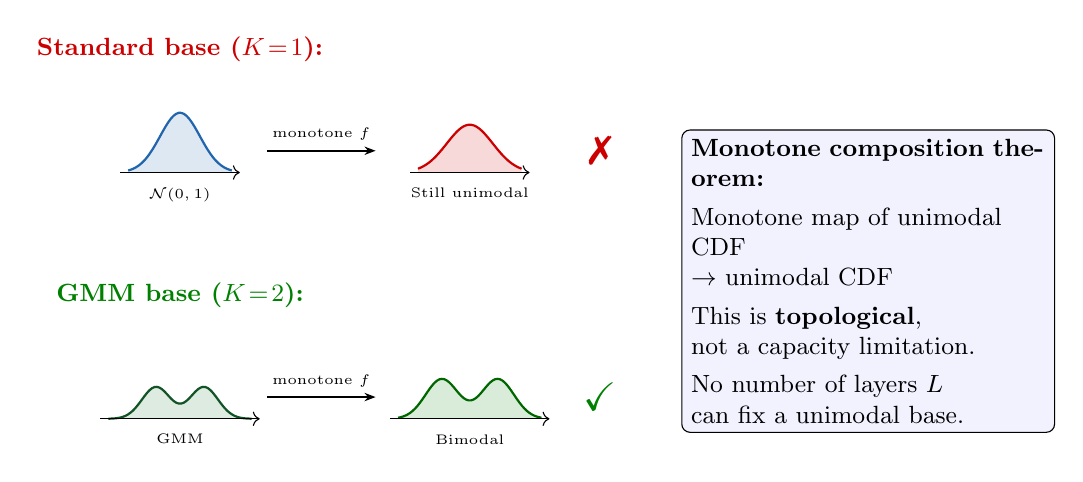
\begin{tikzpicture}[
    box/.style={draw,rounded corners=2pt,minimum width=1.6cm,minimum height=0.7cm,
                align=center,font=\scriptsize},
    arr/.style={-{Stealth[length=4pt]},thick},
    scale=0.92
]
  % === TOP ROW: Standard base (FAILS) ===
  \node[font=\small\bfseries,color=alertred] at (-4.5,2.2) {Standard base ($K\!=\!1$):};

  % Gaussian base
  \begin{scope}[shift={(-4.5,0.5)},scale=0.55]
    \fill[datablue!15] (-1.3,0) -- plot[domain=-1.3:1.3,samples=40]
      (\x, {1.5*exp(-2*\x*\x)}) -- (1.3,0) -- cycle;
    \draw[thick,datablue,domain=-1.3:1.3,samples=40]
      plot (\x, {1.5*exp(-2*\x*\x)});
    \draw[->] (-1.5,0) -- (1.5,0);
    \node[below,font=\tiny] at (0,-0.15) {$\mathcal{N}(0,1)$};
  \end{scope}

  \draw[arr] (-3.3,0.8) -- (-1.8,0.8) node[midway,above,font=\tiny] {monotone $f$};

  % Still unimodal
  \begin{scope}[shift={(-0.5,0.5)},scale=0.55]
    \fill[alertred!15] (-1.3,0) -- plot[domain=-1.3:1.3,samples=40]
      (\x, {1.2*exp(-1.5*\x*\x)}) -- (1.3,0) -- cycle;
    \draw[thick,alertred,domain=-1.3:1.3,samples=40]
      plot (\x, {1.2*exp(-1.5*\x*\x)});
    \draw[->] (-1.5,0) -- (1.5,0);
    \node[below,font=\tiny] at (0,-0.15) {Still unimodal};
  \end{scope}

  \node[font=\Large,color=alertred] at (1.3,0.8) {\ding{55}};

  % === BOTTOM ROW: GMM base (WORKS) ===
  \node[font=\small\bfseries,color=successgreen] at (-4.5,-1.2) {GMM base ($K\!=\!2$):};

  % GMM base
  \begin{scope}[shift={(-4.5,-2.9)},scale=0.55]
    \fill[nfgreen!15] (-1.8,0) -- plot[domain=-1.8:1.8,samples=60]
      (\x, {0.8*exp(-4*(\x-0.6)*(\x-0.6)) + 0.8*exp(-4*(\x+0.6)*(\x+0.6))}) -- (1.8,0) -- cycle;
    \draw[thick,nfgreen!70!black,domain=-1.8:1.8,samples=60]
      plot (\x, {0.8*exp(-4*(\x-0.6)*(\x-0.6)) + 0.8*exp(-4*(\x+0.6)*(\x+0.6))});
    \draw[->] (-2.0,0) -- (2.0,0);
    \node[below,font=\tiny] at (0,-0.15) {GMM};
  \end{scope}

  \draw[arr] (-3.3,-2.6) -- (-1.8,-2.6) node[midway,above,font=\tiny] {monotone $f$};

  % Bimodal target
  \begin{scope}[shift={(-0.5,-2.9)},scale=0.55]
    \fill[successgreen!15] (-1.8,0) -- plot[domain=-1.8:1.8,samples=60]
      (\x, {1.0*exp(-3*(\x-0.7)*(\x-0.7)) + 1.0*exp(-3*(\x+0.7)*(\x+0.7))}) -- (1.8,0) -- cycle;
    \draw[thick,successgreen!80!black,domain=-1.8:1.8,samples=60]
      plot (\x, {1.0*exp(-3*(\x-0.7)*(\x-0.7)) + 1.0*exp(-3*(\x+0.7)*(\x+0.7))});
    \draw[->] (-2.0,0) -- (2.0,0);
    \node[below,font=\tiny] at (0,-0.15) {Bimodal};
  \end{scope}

  \node[font=\Large,color=successgreen] at (1.3,-2.6) {\checkmark};

  % Explanation box on the right
  \node[draw,rounded corners=3pt,fill=blue!5,text width=4.5cm,align=left,font=\small]
    at (5.0,-1.0) {
    \textbf{Monotone composition theorem:}\\[0.3em]
    Monotone map of unimodal CDF\\
    $\to$ unimodal CDF\\[0.3em]
    This is \textbf{topological},\\not a capacity limitation.\\[0.3em]
    No number of layers $L$\\can fix a unimodal base.
  };
\end{tikzpicture}

\end{frame}

% ============================================================================
\section{Validation}
% ============================================================================

\begin{frame}{Validation 1: Equilibrium ($h = 0$)}

\centering
\includegraphics[width=0.92\textwidth]{fig1_equilibrium_validation.pdf}

\smallskip
\begin{columns}[T]
\column{0.32\textwidth}
\centering
{\small (a) NF $\approx$ Boltzmann\\$D_{\mathrm{KL}} \approx \num{0.002}$}

\column{0.32\textwidth}
\centering
{\small (b) Score matches\\$-V'(x)/\kB T$}

\column{0.32\textwidth}
\centering
{\small (c) EPR $\Sigma \approx 0.14 \approx 0$\\(detailed balance $\checkmark$)}
\end{columns}

\end{frame}

% ============================================================================

\begin{frame}{Validation 2: Harmonic Potential}

\centering
\includegraphics[width=0.70\textwidth]{fig2_harmonic_validation.pdf}

\smallskip
\begin{itemize}
    \item $V(x) = kx^2/2$, $k = 2$, $\kB T = 0.5$ $\implies$ $p(x) = \mathcal{N}(0,\, 0.5)$
    \item $D_{\mathrm{KL}} \approx \num{0.0014}$; residual bounded within $\pm\num{0.01}$
    \item Confirms negligible systematic bias for unimodal targets
\end{itemize}

\end{frame}

% ============================================================================
\section{Results}
% ============================================================================

\begin{frame}{Learned Density Tracks the Driven Protocol}

\centering
\includegraphics[width=0.80\textwidth]{fig3_learned_density_snapshots.pdf}

\smallskip
{\small NF (dashed) vs Boltzmann (solid) at $h = -2, -1, 0, +1, +2$.
Deviations reflect non-equilibrium lag.}

\end{frame}

% ============================================================================

\begin{frame}{Main Result: EPR Decomposition}

\centering
\includegraphics[width=0.65\textwidth,trim=0 250 0 0,clip]{fig4_epr_nf_vs_sekimoto.pdf}

\smallskip
{\small (a) Protocol $h(t)$ and response $\langle x\rangle(t)$.
(b) EPR: Sekimoto total (black), NF (blue), Schnakenberg CG (red dashed).}

\end{frame}

% ============================================================================

\begin{frame}{EPR Decomposition -- Key Numbers}

\begin{columns}[T]
\column{0.45\textwidth}
\textbf{Cycle-integrated entropy production:}

\smallskip
\begin{tabular}{lrl}
\toprule
\textbf{Method} & $\boldsymbol{\Sigma}$ & \textbf{Fraction} \\
\midrule
Sekimoto (total) & 10.49 & 100\% \\
\textbf{NF (this work)} & \textbf{11.41} & \textbf{109\%} \\
Schnakenberg (CG) & 0.47 & 4.5\% \\
\bottomrule
\end{tabular}

\smallskip
{\small Slight overshoot from tail noise\\in finite-difference score estimation.}

\column{0.50\textwidth}
\textbf{What the NF method captures:}

\smallskip
\begin{itemize}
    \item Intrawell relaxation currents
    \item Transient probability redistribution
    \item Near-spinodal dissipation peaks
    \item Full spatiotemporal EPR field $\sigma(x,t)$
\end{itemize}

\smallskip
\smallemphbox{
\centering
\textbf{Schnakenberg misses 95\%}\\
\textbf{NF recovers it all}
}
\end{columns}

\end{frame}

% ============================================================================

\begin{frame}{Architecture Comparison: Standard vs GMM Base}

\centering
\includegraphics[width=0.90\textwidth]{fig5_architecture_comparison.pdf}

\smallskip
{\small (a) Standard base: unimodal fit, $D_{\mathrm{KL}}\!\sim\!0.15$--$0.33$.
(b) Wrong score shape.
(c) KL vs layers: GMM $\sim\!0.002$ for all $L\!\geq\!4$.}

\end{frame}

% ============================================================================

\begin{frame}{GMM Base: Quantitative Comparison}

\centering
\begin{tabular}{lcc}
\toprule
& \textbf{Standard normal ($K\!=\!1$)} & \textbf{GMM ($K\!=\!2$)} \\
\midrule
$D_{\mathrm{KL}}$ at $L=4$ & $\sim 0.33$ & $\sim 0.002$ \\
$D_{\mathrm{KL}}$ at $L=12$ & $\sim 0.15$ & $\sim 0.002$ \\
$D_{\mathrm{KL}}$ at $L=20$ & $\sim 0.15$ & $\sim 0.002$ \\
\midrule
Bimodal density? & \textcolor{alertred}{Never} & \textcolor{successgreen}{Always} \\
Score accurate? & \textcolor{alertred}{No} & \textcolor{successgreen}{Yes} \\
EPR reliable? & \textcolor{alertred}{No} & \textcolor{successgreen}{Yes} \\
\bottomrule
\end{tabular}

\vspace{0.8em}
\emphbox{
\centering
\textbf{Practical rule:} Any monotone NF architecture (planar, Real-NVP in 1D)\\
requires a multimodal base when the target density is multimodal.
}

\end{frame}

% ============================================================================
\section{Discussion}
% ============================================================================

\begin{frame}{Step 1: Learning the Density with Normalizing Flows}

\centering
\textbf{This stage is shared by both NF-EPR and Force-Free methods}

\vspace{0.8em}
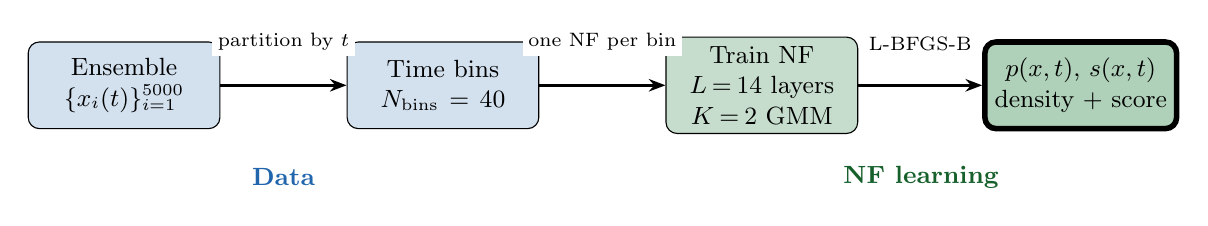
\begin{tikzpicture}[
    box/.style={draw,rounded corners=4pt,minimum height=1.1cm,
                align=center,font=\small,text width=2.2cm},
    arr/.style={-{Stealth[length=6pt]},thick,line width=1.2pt},
    lbl/.style={font=\scriptsize,align=center,fill=white,inner sep=2pt},
    scale=0.9
]
  % Boxes
  \node[box,fill=datablue!20] (ens) at (0,0) {Ensemble\\$\{x_i(t)\}_{i=1}^{5000}$};
  \node[box,fill=datablue!20] (bins) at (4.5,0) {Time bins\\$N_{\mathrm{bins}}=40$};
  \node[box,fill=nfgreen!25] (nf) at (9,0) {Train NF\\$L\!=\!14$ layers\\$K\!=\!2$ GMM};
  \node[box,fill=nfgreen!35,line width=2pt] (dens) at (13.5,0) {$p(x,t)$, $s(x,t)$\\density + score};

  % Arrows
  \draw[arr] (ens) -- (bins) node[midway,above=10pt,lbl] {partition by $t$};
  \draw[arr] (bins) -- (nf) node[midway,above=10pt,lbl] {one NF per bin};
  \draw[arr] (nf) -- (dens) node[midway,above=10pt,lbl] {L-BFGS-B};

  % Color legend
  \node[font=\small,datablue] at (2.25,-1.3) {\textbf{Data}};
  \node[font=\small,nfgreen!80!black] at (11.25,-1.3) {\textbf{NF learning}};
\end{tikzpicture}

\vspace{0.6em}
\begin{itemize}
    \item 47 parameters per snapshot ($3L$ flow + $3K\!-\!1$ GMM base)
    \item Score $s(x) = \partial\log p/\partial x$ via finite differences ($\epsilon = 10^{-5}$)
    \item \textbf{Output:} Explicit density $p(x,t)$ at each time snapshot
\end{itemize}

\vspace{0.4em}
\begin{block}{\small Computational cost (pure NumPy/SciPy, single CPU)}
\small
\begin{tabular}{@{}ll@{}}
Langevin simulation (5000 particles, 3 cycles): & $\sim$\SI{7}{s} \\
NF training (40 snapshots $\times$ \SI{40}{s}/model): & $\sim$\SI{27}{min} \\
EPR computation (both methods): & $<$\SI{0.5}{s} \\
\end{tabular}\\[0.2em]
$\Rightarrow$ \textbf{NF training dominates}; force-free adds only \SI{0.4}{s} overhead
\end{block}

\vspace{0.3em}
\emphbox{\centering The learned $p(x,t)$ is the \textbf{foundation} for both EPR methods.}

\end{frame}

% ============================================================================

\begin{frame}{Step 2a: NF--EPR (Requires Known Force)}

\centering
\textbf{Starting from the learned density $p(x,t)$...}

\vspace{0.6em}
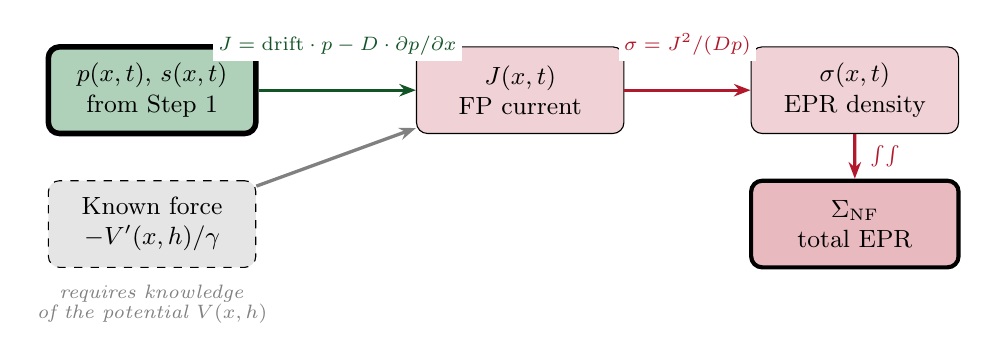
\begin{tikzpicture}[
    box/.style={draw,rounded corners=4pt,minimum height=1.1cm,
                align=center,font=\small,text width=2.4cm},
    arr/.style={-{Stealth[length=6pt]},thick,line width=1.2pt},
    lbl/.style={font=\scriptsize,align=center,fill=white,inner sep=2pt},
    scale=0.85
]
  % Input from Step 1
  \node[box,fill=nfgreen!35,line width=2pt] (dens) at (0,0) {$p(x,t)$, $s(x,t)$\\from Step 1};

  % Known force input
  \node[box,fill=gray!20,dashed] (force) at (0,-2) {Known force\\$-V'(x,h)/\gamma$};

  % Processing
  \node[box,fill=physred!20] (curr) at (5.5,0) {$J(x,t)$\\FP current};
  \node[box,fill=physred!20] (epr) at (10.5,0) {$\sigma(x,t)$\\EPR density};
  \node[box,fill=physred!30,line width=1.5pt] (total) at (10.5,-2) {$\Sigma_{\mathrm{NF}}$\\total EPR};

  % Arrows
  \draw[arr,nfgreen!70!black] (dens) -- (curr) node[midway,above=10pt,lbl] {$J = \mathrm{drift}\cdot p - D\cdot\partial p/\partial x$};
  \draw[arr,gray] (force) -- (curr);
  \draw[arr,physred] (curr) -- (epr) node[midway,above=10pt,lbl] {$\sigma = J^2/(Dp)$};
  \draw[arr,physred] (epr) -- (total) node[midway,right=3pt,lbl] {$\int\!\int$};

  % Annotation
  \node[font=\scriptsize,gray,align=center] at (0,-3.2) {\textit{requires knowledge}\\[-0.1em]\textit{of the potential $V(x,h)$}};
\end{tikzpicture}

\vspace{0.5em}
\begin{columns}[T]
\column{0.48\textwidth}
\textbf{Fokker--Planck current:}
$$J = -\frac{V'(x,h)}{\gamma}p - D\frac{\partial p}{\partial x}$$

\column{0.48\textwidth}
\textbf{Result:}\\
$\Sigma_{\mathrm{NF}} = 10.87$ (3.6\% error vs Sekimoto)
\end{columns}

\end{frame}

% ============================================================================

\begin{frame}{Positioning in the Literature}

\centering
\begin{tabular}{l c c c}
\toprule
\textbf{Method} & \textbf{Output} & \textbf{Density} & \textbf{Time-dep.} \\
\midrule
NEEP (Kim et al., 2020) & Scalar bound & Implicit & No \\
Score-based (Boffi et al., 2024) & $\sigma(\mathbf{x})$ field & Implicit & Steady only \\
Temporal NF (Feng et al., 2022) & $p(x,t)$ & Explicit & Yes \\
Score-PINN (Hu et al., 2024) & $p(x,t)$ & Via score & Yes \\
\midrule
\textbf{This work} & $\boldsymbol{\sigma(x,t)}$ \textbf{field} & \textbf{Explicit} & \textbf{Yes} \\
\bottomrule
\end{tabular}

\vspace{0.8em}
\begin{columns}[T]
\column{0.48\textwidth}
\textbf{vs.\ Score-based (Boffi):}
\begin{itemize}
    \item We provide \emph{explicit} $p(x,t)$
    \item We track \emph{driven} protocols
    \item They scale to high-D (transformers)
\end{itemize}

\column{0.48\textwidth}
\textbf{vs.\ Temporal NF (Feng):}
\begin{itemize}
    \item They train on FP loss directly
    \item We train snapshot-by-snapshot
    \item We compute EPR, not just $p(x,t)$
\end{itemize}
\end{columns}

\vspace{0.3em}
\emphbox{
\centering
\textbf{First explicit-density NF method} for time-resolved EPR in driven systems.
}

\end{frame}

% ============================================================================

\begin{frame}{Limitations and Future Directions}

\begin{columns}[T]
\column{0.48\textwidth}
\textbf{Limitations:}
\begin{itemize}
    \item \textbf{1D only} -- higher dimensions need coupling layers
    \item \textbf{Pure NumPy} -- score via finite differences
    \item \textbf{Independent snapshots} -- temporal correlations discarded
    \item \textbf{Known dynamics} -- \textcolor{successgreen}{resolved} via continuity eq.\ (next section)
\end{itemize}

\column{0.48\textwidth}
\textbf{Extensions:}
\begin{itemize}
    \item Experimental data (colloids, motors)
    \item Higher-D flows (Real-NVP, FFJORD)
    \item Conditional flow $p(x|t)$
    \item Thermodynamic uncertainty relations
\end{itemize}
\end{columns}

\end{frame}

% ============================================================================

\begin{frame}{Companion Paper}

\begin{columns}[T]
\column{0.48\textwidth}
\emphbox{
\textit{``Topological Hysteresis Bounds and Hidden Entropy in Driven Landau Theory''}\\[0.2em]
{\small Fern\'andez-Caballero (2026)}
}

\smallskip
\textbf{Established:}
\begin{itemize}
    \item $\mathcal{W}_{\max} = 6.0$ upper bound
    \item Schnakenberg $\sim$4--6\% of total
    \item $\sim$95\% hidden intrawell entropy
\end{itemize}

\column{0.48\textwidth}
\vspace{1.5em}
\textbf{This paper closes the circle:}
\begin{itemize}
    \item Hidden fraction \textbf{recovered} via NF density estimation
    \item No analytical density needed -- learned from trajectory data
    \item Same physical system, complementary methodology
\end{itemize}
\end{columns}

\end{frame}

% ============================================================================
\section{Force-Free Extension}
\label{sec:forcefree}
% ============================================================================

\begin{frame}{Step 2b: Force-Free Pipeline (No Force Required)}

\centering
\textbf{Starting from the learned density $p(x,t)$...}

\vspace{0.6em}
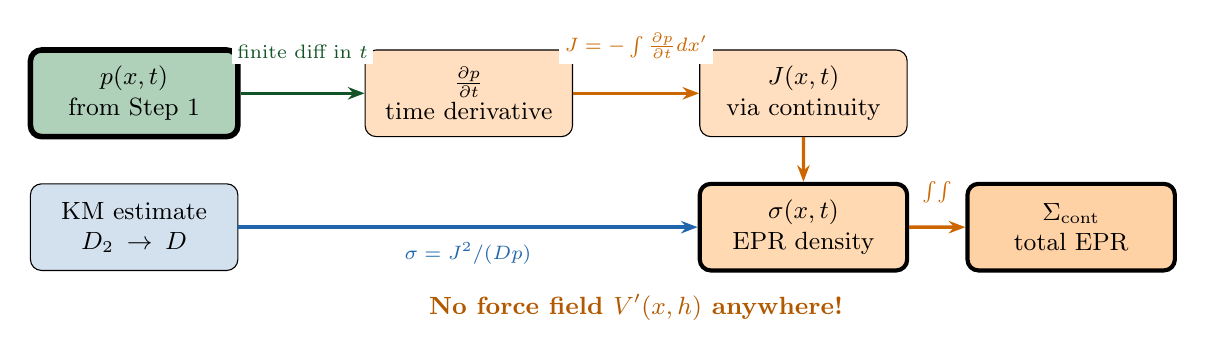
\begin{tikzpicture}[
    box/.style={draw,rounded corners=4pt,minimum height=1.1cm,
                align=center,font=\small,text width=2.4cm},
    arr/.style={-{Stealth[length=6pt]},thick,line width=1.2pt},
    lbl/.style={font=\scriptsize,align=center,fill=white,inner sep=2pt},
    scale=0.85
]
  % Input from Step 1
  \node[box,fill=nfgreen!35,line width=2pt] (dens) at (0,0) {$p(x,t)$\\from Step 1};

  % KM estimate for D
  \node[box,fill=datablue!20] (km) at (0,-2) {KM estimate\\$D_2 \to D$};

  % Processing - continuity equation path
  \node[box,fill=orange!25] (dpdt) at (5,0) {$\frac{\partial p}{\partial t}$\\time derivative};
  \node[box,fill=orange!25] (curr) at (10,0) {$J(x,t)$\\via continuity};
  \node[box,fill=orange!30,line width=1.5pt] (epr) at (10,-2) {$\sigma(x,t)$\\EPR density};
  \node[box,fill=orange!35,line width=1.5pt] (total) at (14,-2) {$\Sigma_{\mathrm{cont}}$\\total EPR};

  % Arrows
  \draw[arr,nfgreen!70!black] (dens) -- (dpdt) node[midway,above=10pt,lbl] {finite diff in $t$};
  \draw[arr,orange!80!black] (dpdt) -- (curr) node[midway,above=10pt,lbl] {$J = -\int \frac{\partial p}{\partial t}dx'$};
  \draw[arr,orange!80!black] (curr) -- (epr);
  \draw[arr,datablue] (km) -- (epr) node[midway,below=3pt,lbl] {$\sigma = J^2/(Dp)$};
  \draw[arr,orange!80!black] (epr) -- (total) node[midway,above=6pt,lbl] {$\int\!\int$};

  % Annotation - no force!
  \node[font=\small,orange!70!black,align=center] at (7.5,-3.2) {\textbf{No force field $V'(x,h)$ anywhere!}};
\end{tikzpicture}

\vspace{0.4em}
\begin{columns}[T]
\column{0.48\textwidth}
\textbf{Key insight:} Fokker--Planck is a continuity equation
$$\frac{\partial p}{\partial t} = -\frac{\partial J}{\partial x}$$
Integrate to get $J$ without knowing the force!

\column{0.48\textwidth}
\textbf{Result:}\\
$\Sigma_{\mathrm{cont}} = 9.31$ (11.3\% error vs Sekimoto)\\[0.3em]
\textit{Only $D$ required as input}
\end{columns}

\end{frame}

% ============================================================================

\begin{frame}{Comparing the Two Approaches}

\centering
\vspace{0.3em}
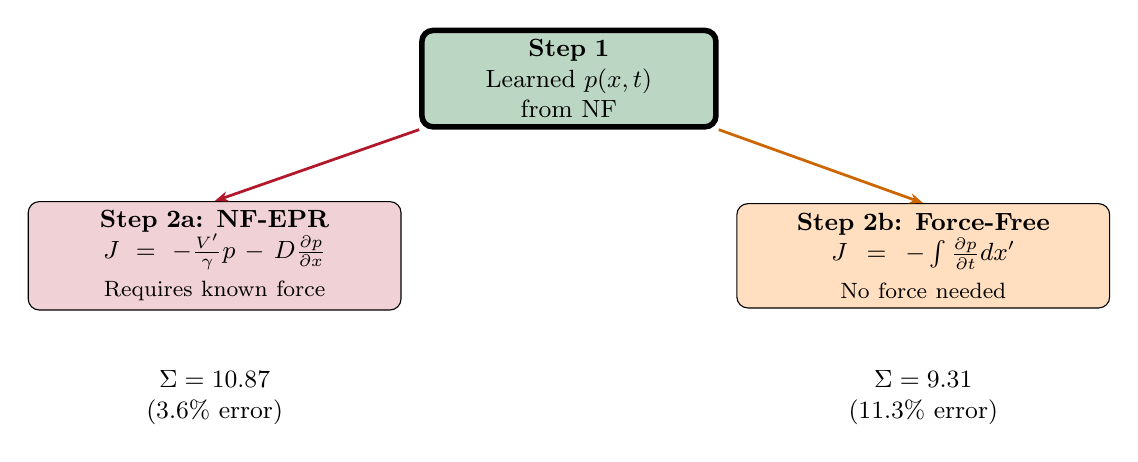
\begin{tikzpicture}[
    box/.style={draw,rounded corners=4pt,minimum height=1cm,
                align=center,font=\small},
    arr/.style={-{Stealth[length=5pt]},thick,line width=1pt},
    scale=0.9
]
  % Shared foundation
  \node[box,fill=nfgreen!30,line width=2pt,text width=3.5cm] (dens) at (0,0) {\textbf{Step 1}\\Learned $p(x,t)$\\from NF};

  % Two paths
  \node[box,fill=physred!20,text width=4.5cm] (nfepr) at (-5,-2.5) {\textbf{Step 2a: NF-EPR}\\$J = -\frac{V'}{\gamma}p - D\frac{\partial p}{\partial x}$\\[0.3em]\footnotesize Requires known force};

  \node[box,fill=orange!25,text width=4.5cm] (ff) at (5,-2.5) {\textbf{Step 2b: Force-Free}\\$J = -\int \frac{\partial p}{\partial t}dx'$\\[0.3em]\footnotesize No force needed};

  % Arrows from shared to paths
  \draw[arr,physred] (dens.south west) -- (nfepr.north);
  \draw[arr,orange!80!black] (dens.south east) -- (ff.north);

  % Results
  \node[font=\small,align=center] at (-5,-4.5) {$\Sigma = 10.87$\\(3.6\% error)};
  \node[font=\small,align=center] at (5,-4.5) {$\Sigma = 9.31$\\(11.3\% error)};

\end{tikzpicture}

\vspace{0.5em}
\emphbox{
\centering
\textbf{Both methods share the NF density learning (Step 1)}\\[0.2em]
Force-free trades accuracy (11\% vs 4\%) for \textbf{broader applicability}\\
(works when the force field is unknown)
}

\end{frame}

% ============================================================================

\begin{frame}{Force-Free Validation (Fig.\ 6)}

\centering
\includegraphics[width=0.52\textwidth]{fig6_km_epr_comparison.pdf}

\smallskip
{\small (a) KM drift vs known: good in core, noisy in tails.
(b) $\langle D_2\rangle = 0.554$ ($10.8\%$ above true $D$).
(c) Continuity EPR tracks NF shape, systematic undershoot.
(d) Integrated: $\Sigma_{\mathrm{cont}} = 9.3$ ($11.3\%$ error).}

\end{frame}

% ============================================================================

\begin{frame}{Force-Free EPR: Key Numbers}

\centering
\begin{tabular}{lrl}
\toprule
\textbf{Method} & $\boldsymbol{\Sigma}$ & \textbf{Error vs Sekimoto} \\
\midrule
Sekimoto (reference) & 10.49 & --- \\
NF (known force) & 10.87 & 3.6\% \\
\textbf{Continuity (force-free)} & \textbf{9.31} & \textbf{11.3\%} \\
Schnakenberg (CG) & 0.47 & 95.5\% \\
\bottomrule
\end{tabular}

\vspace{1.0em}
\emphbox{
\centering
\textbf{Force-free estimate within 12\%} --- no dynamics required.\\[0.3em]
Only the diffusion coefficient $D$ (from KM $D_2$) is needed.
}

\vspace{0.8em}
{\small Undershoot from finite temporal resolution in $\partial p/\partial t$ ($N_{\mathrm{bins}} = 20$).\\
Increasing temporal resolution would improve accuracy systematically.}

\end{frame}

% ============================================================================
\section{Conclusions}
% ============================================================================

\begin{frame}{Conclusions}

\begin{enumerate}
    \item \textbf{NF-EPR recovers the full dissipation:}\\
    $\Sigma_{\mathrm{NF}} \approx 11.4$ agrees with $\Sigma_{\mathrm{Sek}} \approx 10.5$ to within 10\%\\
    (vs $\Sigma_{\mathrm{CG}} \approx 0.5$, or $\sim$5\% of total)

    \vspace{0.4em}
    \item \textbf{GMM base is essential for bimodal targets:}\\
    Monotone composition theorem: unimodal base $\to$ unimodal output\\
    $K=2$ GMM resolves both wells with $D_{\mathrm{KL}} \sim 0.002$

    \vspace{0.4em}
    \item \textbf{Force-free EPR via continuity equation:}\\
    $\Sigma_{\mathrm{cont}} = 9.3$ ($11.3\%$ error) --- no dynamics required,\\
    only the diffusion coefficient $D$ from KM estimation

    \vspace{0.4em}
    \item \textbf{Accessible implementation:}\\
    Pure NumPy/SciPy, 47 parameters per snapshot\\
    Suitable for teaching and small-scale research
\end{enumerate}

\vspace{0.3em}
\centering
\textbf{Code:} \texttt{Markov\_Chains\_MC/NF\_Langevin/}

\end{frame}

% ============================================================================

\begin{frame}{}
\centering
\vspace{2cm}
{\Huge Thank you}

\vspace{1.5cm}
{\large Antonio Fern\'{a}ndez-Caballero}\\[0.3em]
{\normalsize \texttt{antonio.fcaballero@urjc.es}}\\[0.3em]
{\normalsize URJC -- LEADS / BigMed+}
\end{frame}

% ============================================================================
% BACKUP SLIDES
% ============================================================================

\appendix

\begin{frame}{Backup Slides}
\centering
{\Large Additional Material}
\end{frame}

% ============================================================================

\begin{frame}{Simulation Parameters}

\centering
\begin{tabular}{lcl}
\toprule
\textbf{Parameter} & \textbf{Value} & \textbf{Description} \\
\midrule
$\gamma$ & 1.0 & Friction coefficient \\
$\kB T$ & 0.5 & Thermal energy \\
$D = \kB T/\gamma$ & 0.5 & Diffusion coefficient \\
$\Delta t$ & 0.002 & Euler--Maruyama time step \\
$h_{\max}$ & 2.0 & Driving amplitude \\
$\mathcal{T}$ & \SI{10}{s} & Driving period \\
$N$ & 5000 & Ensemble size \\
Transient & 5 cycles & Discarded before analysis \\
Analysis & 6th cycle & Non-equilibrium steady state \\
Seed & 42 & Reproducibility \\
\bottomrule
\end{tabular}

\end{frame}

% ============================================================================

\begin{frame}{Euler--Maruyama Discretization}

\begin{equation*}
    x(t+\Delta t) = x(t) - \frac{V'(x,h)}{\gamma}\,\Delta t + \sqrt{2D\,\Delta t}\;\eta(t)
\end{equation*}

where $\eta(t) \sim \mathcal{N}(0,1)$ are independent Gaussian variates.

\vspace{0.5em}
\textbf{Implementation details:}
\begin{itemize}
    \item Initial positions: $x_0 \in \{-1, +1\}$ with equal probability
    \item Seeded RNG: \texttt{numpy.random.default\_rng(42)}
    \item \num{30000} time steps per cycle, vectorized over $N = \num{5000}$
\end{itemize}

\end{frame}

% ============================================================================

\begin{frame}{Change of Variables Formula}

For $L$ planar layers $f = g_L \circ \cdots \circ g_1$:
\begin{equation*}
    \log p(y) = \log p_Z\!\big(f^{-1}(y)\big) - \sum_{l=1}^{L} \log\left|\frac{dg_l}{dx}\right|_{x=z_l}
\end{equation*}

\textbf{Inversion:} Newton's method on $g_l(x) = y_l$
\begin{itemize}
    \item Converges to $\mathrm{tol} = 10^{-12}$ within 50 iterations
    \item Monotonicity ($u\,w > -1$) guarantees convergence
\end{itemize}

\textbf{Score function:} Central finite differences
\begin{equation*}
    s(x) = \frac{\log p(x+\epsilon) - \log p(x-\epsilon)}{2\epsilon}, \quad \epsilon = 10^{-5}
\end{equation*}

\end{frame}

% ============================================================================

\begin{frame}{Neural ODE: Why It Failed}

\textbf{Neural ODE:} $dx/dt = F(x,t)$, $d(\log p)/dt = -dF/dx$

\smallskip
\begin{columns}[T]
\column{0.48\textwidth}
\textbf{Appealing because:}
\begin{itemize}
    \item Can create/annihilate modes
    \item Direct FP connection
    \item Not monotone-constrained
\end{itemize}

\column{0.48\textwidth}
\textbf{Failed in pure NumPy:}
\begin{itemize}
    \item $n_{\mathrm{params}}+1$ ODE solves per gradient
    \item GMM base: NLL diverged
    \item $>$25 min for 50 samples
    \item Needs AD (PyTorch/JAX)
\end{itemize}
\end{columns}

\end{frame}

\end{document}
